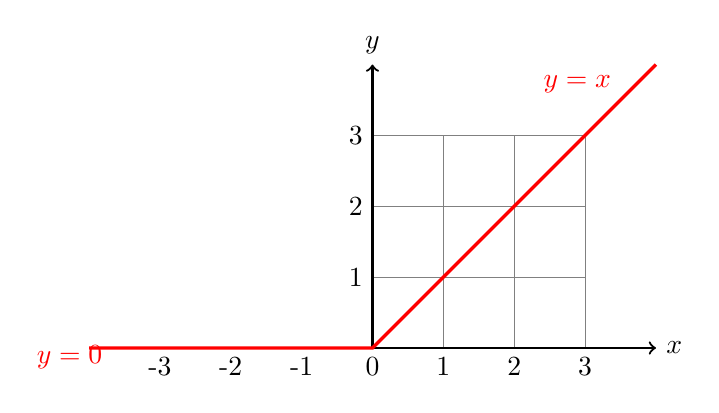
\begin{tikzpicture}[domain=-4:4, scale=.9]
	% grid
	\draw[very thin, color=gray] (0, 0) grid (3, 3);
	
	% axes
	\draw[->,thick] (-4, 0) -- (4, 0) node[right] {$x$};
	\draw[->,thick] (0, 0) -- (0, 4) node[above] {$y$};
	\foreach \x in {-3, ..., 3}
		\node[anchor=north] at (\x, 0) {\x};
	\foreach \y in {1, ..., 3}
		\node[anchor=east] at (0, \y) {\y};
		
	% relu function
	\draw[very thick, color=red] plot (\x, { max(0, \x) }) 
		node[anchor=north,  xshift=-1cm] {$y=x$}
		node[anchor=south west, xshift=-8cm, yshift=-4cm] {$y=0$};
\end{tikzpicture}